\section{Colored grid detector}
\label{sec:cgd}

\subsection{Introduction}
\label{sec:cgd:intro}
I needed to get a discretized description of the environment. To do so, 
I built a detector that discretizes the image and calculates the mean 
color of every block of the grid. The detector uses a given list of 
colors and finds for every block the closest colors of this list to his 
mean. This can be used to assign types to blocks as in a maze, each 
different colors represents a different type. (walls, open space, 
target, etc).

\subsection{Detection and drawing}
\label{sec:cgd:algo}
Here is the algorithm described in chronological order.

    \begin{enumerate}
        \item The detector enhance the colors given the saturation and 
                brightness values.
        \item It calculates the mean color of every block.
        \item It draws the mean color as a thick border inside blocks of 
            the raw image
        \item It calculates the closest color from the mean block color
        \item It draws the block color in the edited image (under the raw 
            image)

    \marginpar{
        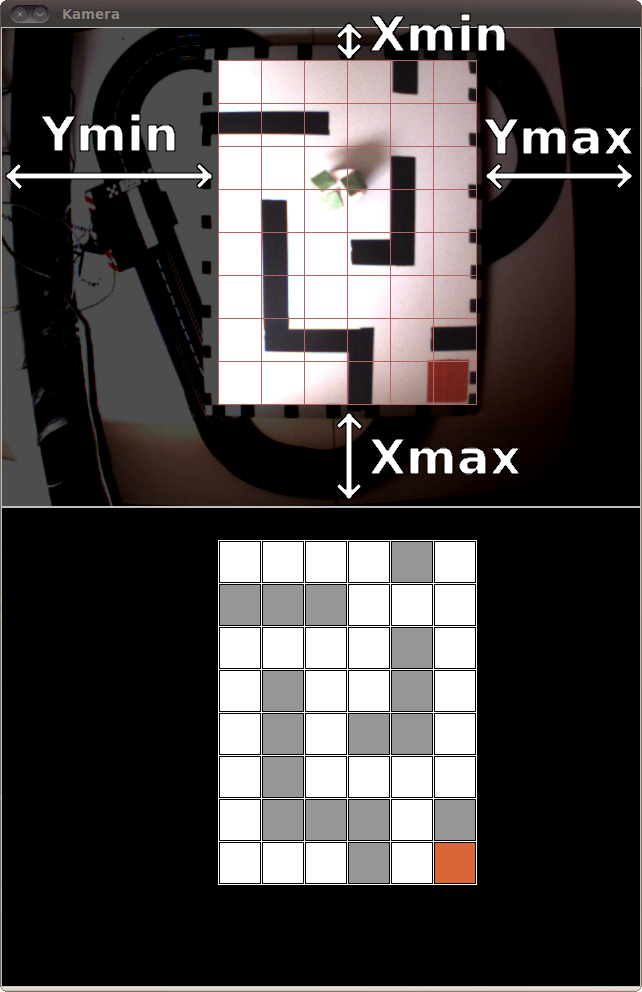
\includegraphics[width=4.5cm]{./img/MazeDetector_minmaxB.png}
        \captionof{figure}[Interface of Colored grid detector]{
        Interface of Colored grid detector -- 
        The subframe can be adjusted to a specific region of the image
        using the $x_{min}$, $x_{max}$, $y_{min}$ and $y_{max}$ values.
        Only this region is considered by the detector.}
        \label{fig:cgd:interface}
    }

        \item It add blocks to the detected objects :
        \begin{itemize}
            \label{sec:cgd:algo:blockattributs}
            \item $x,y$ (upper left corner)
            \item angle=0, size=color index
        \end{itemize}
        \item Draw the grid on the raw an edited image
        \item If in get\_block\_color mode, it draws the mean color of a 
            given block in the edited image.
    \end{enumerate}


\subsection{Improvements}
\label{sec:cgd:improvements}

This is not a major problem, I would even say less serious than 
minor, but the grid is incorrectly drawn when we change the 
min max values of the subframe. It does not happen on start, 
only on live changes. It is sometimes annoying, but it does not 
impact the performance of the detector, neither the usability of it.
\\
\\
It could be useful to change the blocks information mapping 
(point \ref{sec:cgd:algo:blockattributs}. of 
section \ref{sec:cgd:algo}). The color 
index is saved in the size attribute, but we could save the 
actual size of the block, the length of the side, in this attribute. 
Still, for rectangular blocks there would miss an attribute to save 
both side lengths. Even though, the color index could be saved in the 
angle attribute, which his an attribute that,
I think, will never be useful in this context. 

\subsection{How to use}
\label{sec:cgd:howto}
    \begin{enumerate}
        \item Set the $x_{min}$, $x_{max}$, $y_{min}$ and $y_{max}$ 
            values using the arrow keys
            to narrow down the subframe around the environement (maze)
            (see figure \ref{fig:cgd:interface}). Be sure 
            that the terminal has the focus. Print on terminal the values
            by pressing the 'p' key, 
            write it down and save them in the configuration file.
        \item Use the get\_block\_color mode to get the color values (RGB) 
            of specific blocks, so you can give more accurate colors to 
            detect in the configuration file (see 
            figure \ref{fig:cgd:getblockcolor}).
        \item You can adjust the brightness and saturation values to get 
            better results.
    \end{enumerate}

\subsubsection{Parameters config file}
\label{sec:cgd:howto:params}
    \marginpar{
        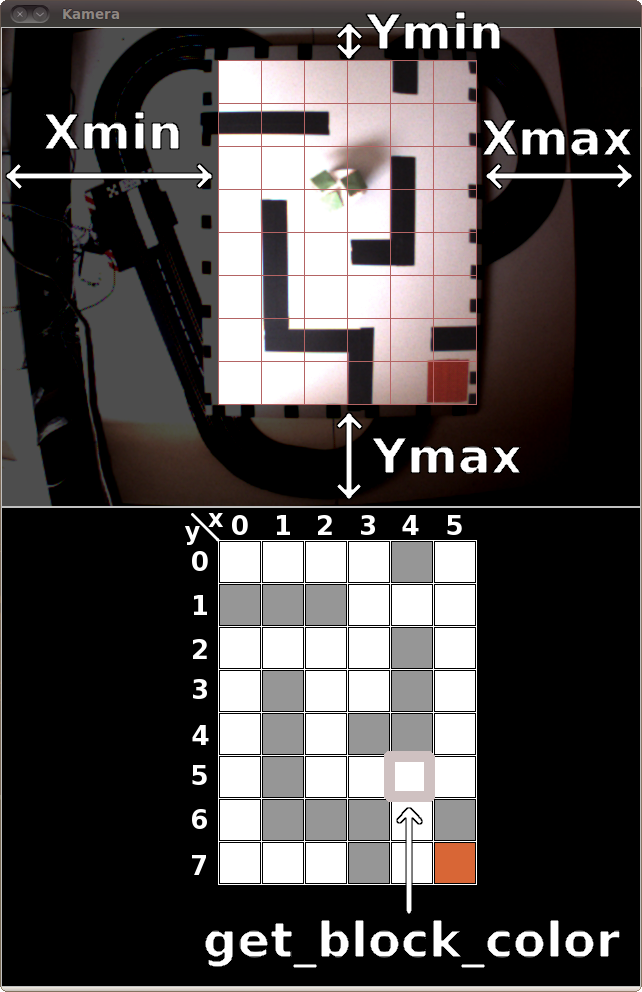
\includegraphics[width=4.5cm]{./img/MazeDetector_get_block_colorB.png}
        \captionof{figure}[Get\_object\_color mode]{%
        Get\_object\_color mode -- 
        This mode is really useful to get mean color value of 
        a given block. The mean color is also drawn as you can 
        see in the image at the end of the arrow.
        }
        \label{fig:cgd:getblockcolor}
    }

    \begin{description} \itemindent=-15pt
        \item[grid\_x] \hfill \\ int, Number of blocks in x
        \item[grid\_y] \hfill \\ int,  Number of blocks in y (default = 
            grid\_x)
        \item[x\_min] \hfill \\ int, Lower limit of the detection frame on 
            the image
        \item[x\_max] \hfill \\ int, Upper limit of the detection frame on 
            the image

        \item[y\_min] \hfill \\ int, Left limit of the detection frame on 
            the image
        \item[y\_max] \hfill \\ int, Right limit of the detection frame on 
            the image
        \item[print\_block\_color] \hfill \\ book, Print the mean color of 
            the block on the raw image
        \item[get\_block\_color] \hfill \\ bool, Enable the 
            get\_block\_color on start
        \item[get\_color\_x] \hfill \\ int,  Initial x position of 
            get\_block\_color block
        \item[get\_color\_y] \hfill \\ int,  Initial y position of 
            get\_block\_color block
        \item[saturation] \hfill \\ int,  Modify saturation of the image
        \item[brightness] \hfill \\ int,  Modify brightness of the image
        \item[colors] \hfill \\ int,int,int$|$int,int,int$|$..., 
            given colors to detect in RGB form
    \end{description}

\subsubsection{Keys}
\label{sec:cgd:howto:keys}
    \begin{description} \itemindent=-15pt
        \item['l'] change minimum (left,up) bounds mode \\
            \begin{tabular}{ll}
                {\bf left } & $y_{min}$ -= 2 \\
                {\bf right} & $y_{min}$ += 2 \\
                {\bf up   } & $x_{min}$ -= 2 \\
                {\bf down } & $x_{min}$ += 2 \\
                {\bf 'p'  } & print $x_{min}$, $x_{max}$, $y_{min}$ and $y_{max}$
            \end{tabular}
        \item['u'] change maximum (right,down) bounds mode \\
            \begin{tabular}{ll}
                {\bf left } & $y_{max}$ -= 2 \\
                {\bf right} & $y_{max}$ += 2 \\
                {\bf up   } & $x_{max}$ -= 2 \\
                {\bf down } & $x_{max}$ += 2 \\
                {\bf 'p'  } & print $x_{min}$, $x_{max}$, $y_{min}$ and $y_{max}$ 
            \end{tabular}
        \item['b']  change brightness mode \\
            \begin{tabular}{ll} 
                {\bf left } & -5 to brightness \\
                {\bf down } & -5 to brightness \\
                {\bf right} & +5 to brightness \\
                {\bf up   } & +5 to brightness \\
                {\bf 'p'  } & print brightness value 
            \end{tabular}
        \item['s'] change saturation mode \\
            \begin{tabular}{ll}
                {\bf left } & -2 to saturation \\
                {\bf down } & -2 to saturation \\
                {\bf right} & +2 to saturation \\
                {\bf up   } & +2 to saturation \\
                {\bf 'p'  } & print saturation value \\
            \end{tabular}
        \item['c'] get\_block\_color mode \\
            \begin{tabular}{ll} 
                {\bf left } & move get\_block\_color block to the left  \\
                {\bf right} & move get\_block\_color block to the right \\
                {\bf down } & move get\_block\_color block down \\
                {\bf up   } & move get\_block\_color block up \\
                {\bf 'p'  } & print get\_block\_color block position and 
                              comparisons \\
                            & (distance) with mean color of 
                              the block and \\
                            & the given colors \\
            \end{tabular}
        \item['e'] exit current mode
    \end{description}
